\chapter{Evaluation}
\label{chap:evaluation}
\begin{chapterintro}
In this chapter we will evaluate the game application through the information retrieved after its deployment
\end{chapterintro}

\cleardoublepage
\section{Overview}
In the following sections we will observe the impact that our application has taken after its deployment. We will analyze both Android and iOs application that we have deployed to Google Play and Apple Store respectively.

The metrics used in this chapter have been recovered using \textit{Game Analytics}. Although ideally we should have used Flurry to retrieved the desired metrics to write this chapter, the client restricted Flurry panel access two years after the application deployment.

Game Analytics is a free and powerful analytics tool for game developers, that helps us to understand player behavior and build better games.~\cite{gametrics1} It is natively included within Unity so we are able to access to lots of metrics out of the box.

\section{Acquisition}

In this section we are going to revise the user acquisition. The most important metrics for user acquisition are number and location of installations. These two metrics are by far the easiest way to tell if our application is something that people find valuable.

We have to notice that although our application is free to download, the pack with the physical instrument pieces should be bought in the client physical stores. This physical pack is shown in Figure \ref{fig:instruments-pack}

\begin{figure}[h]
\centering
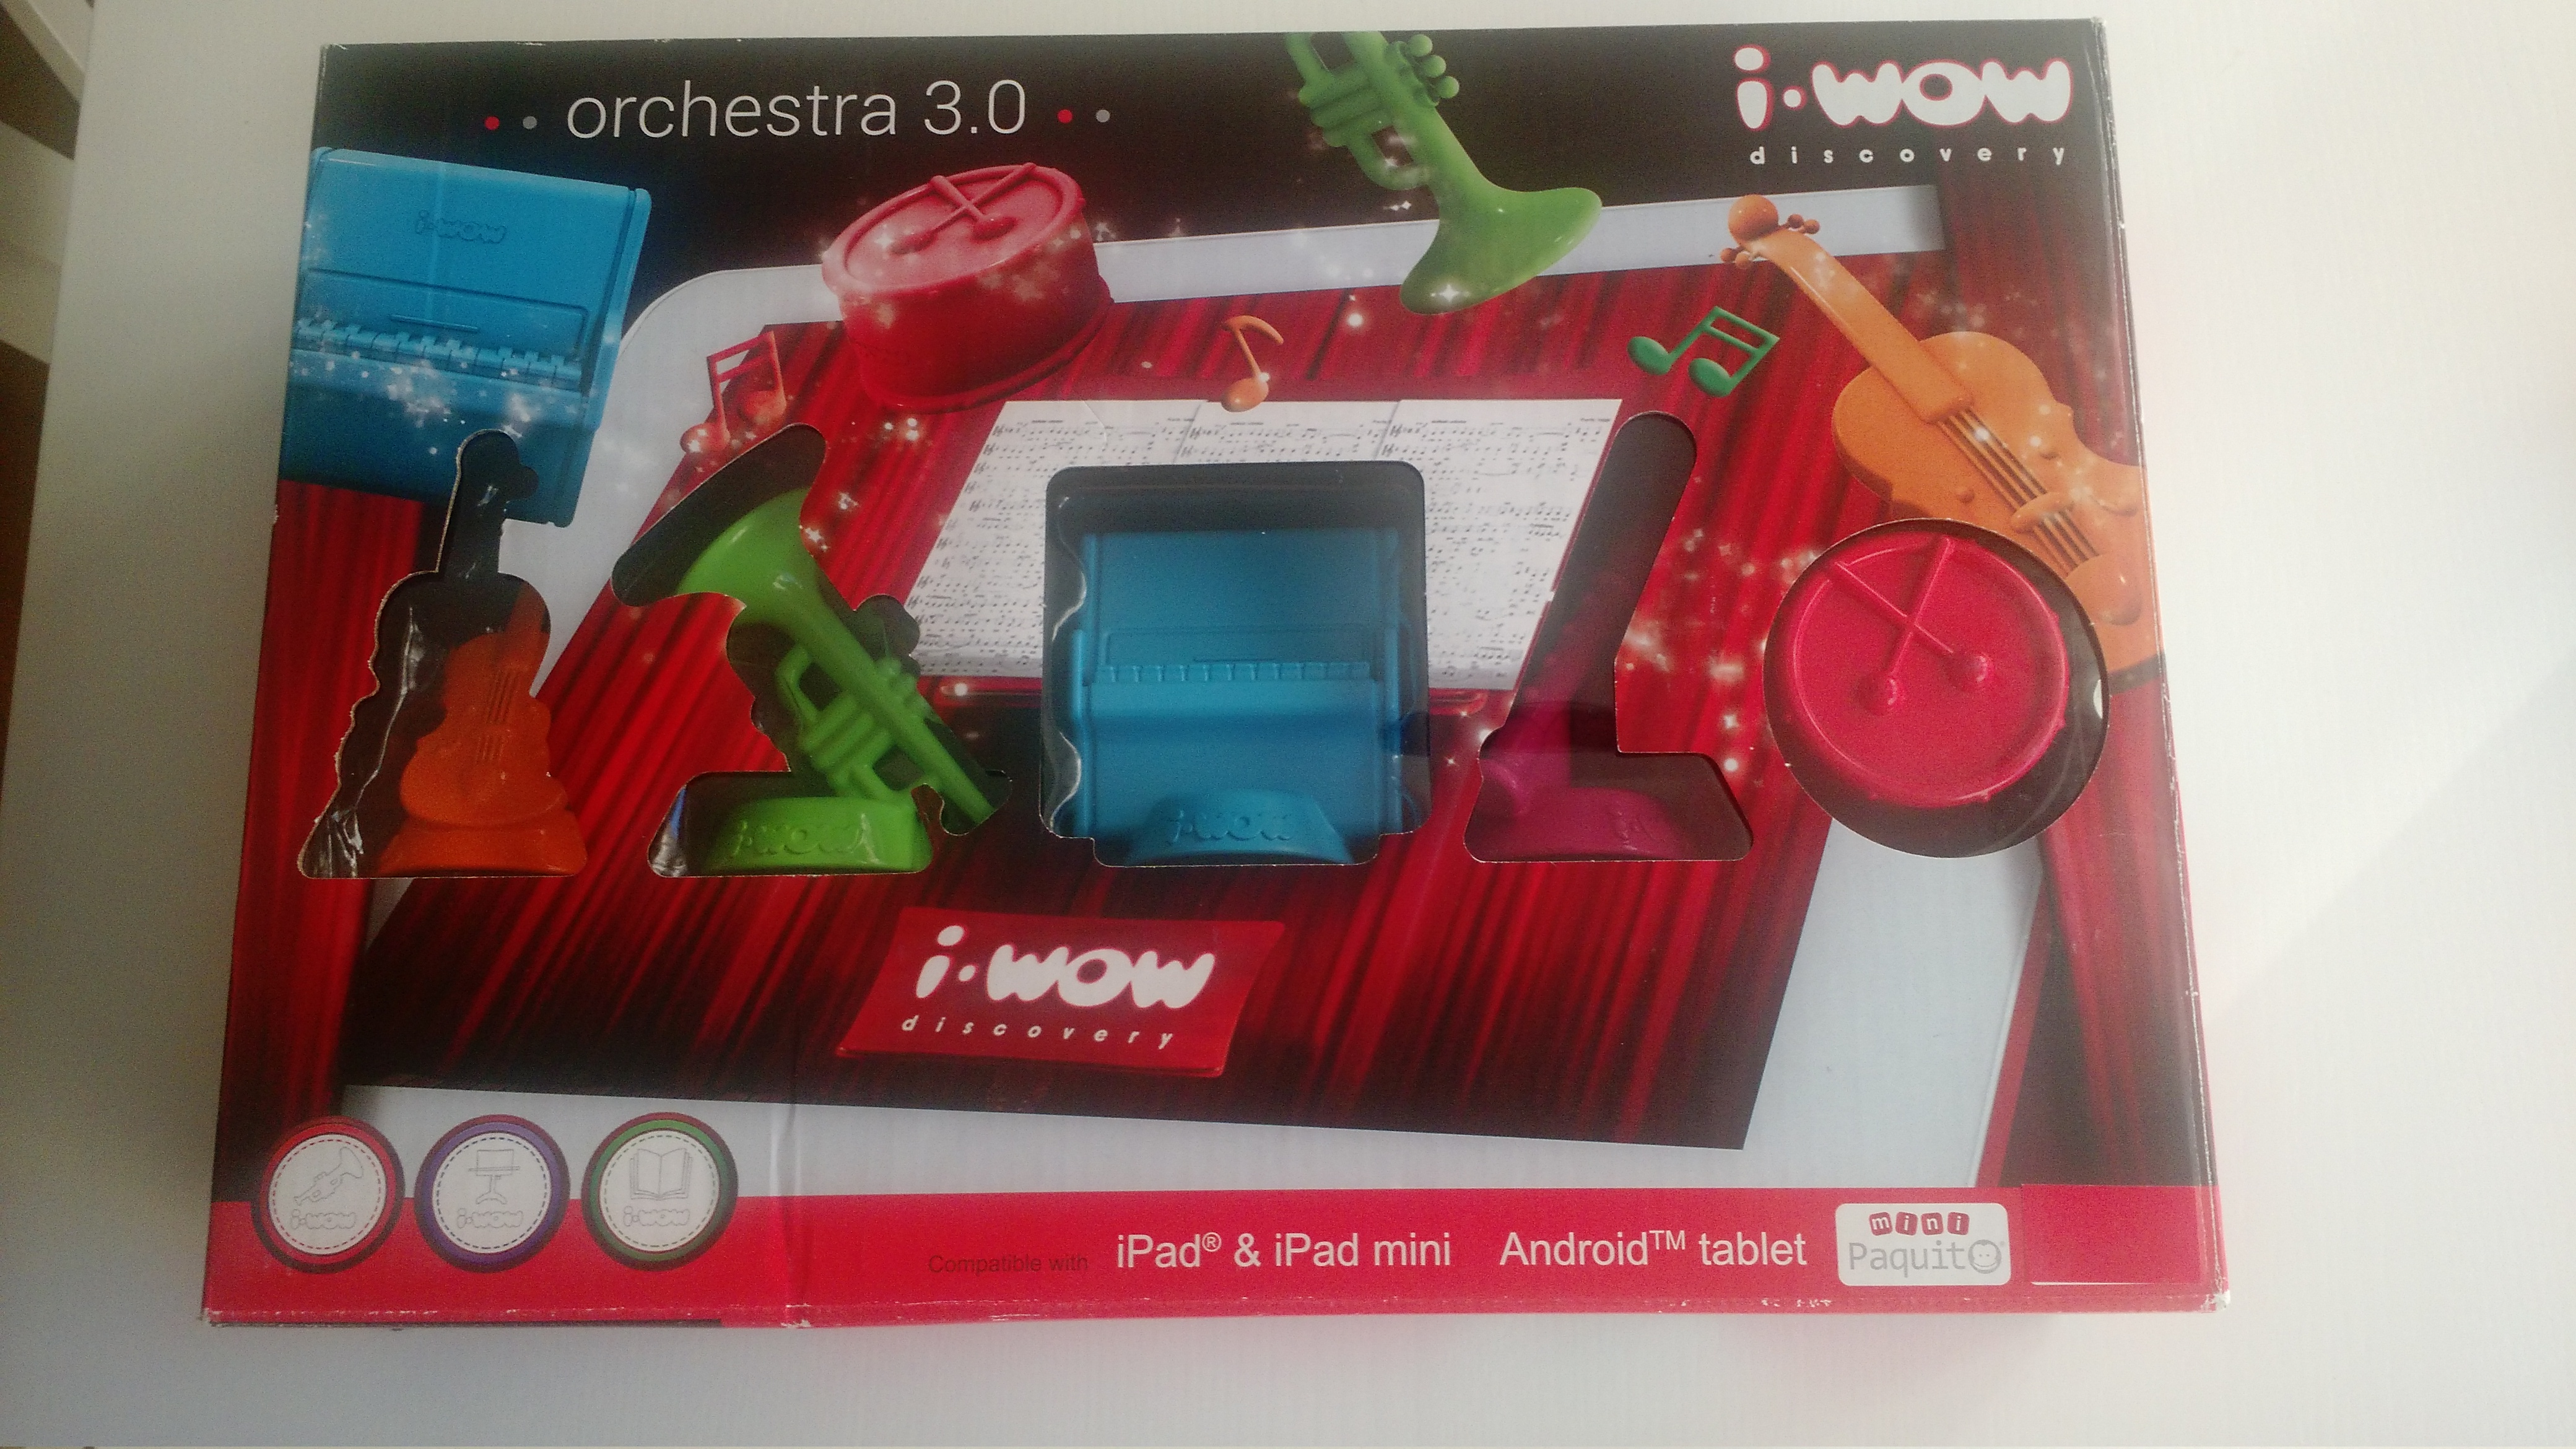
\includegraphics[width=350pt]{graphics/evaluation/instruments_pack.jpg}
\caption{Physical instrument pieces box}
\label{fig:instruments-pack}
\end{figure}

This will impact in the application user acquisition due to the fact that our target users will be the ones who have bought the physical game.

\FloatBarrier

We will study the acquisition metrics in two time periods. Firstly, we will look at the information obtained during the first year since the application was first released, this covers the period between August 2014 and August 2015. Then we will observe the information during the three years that the application has been available on the market which covers the period between August 2014 and February 2017.

\subsection{Number of users}

As we said, one of the most important metrics for user acquisition is the number of installations or the number of users which have download our application in their device.

In Figure \ref{fig:bars-first-year} we can see the new users engaged in the first year:

\begin{figure}[h]
\centering
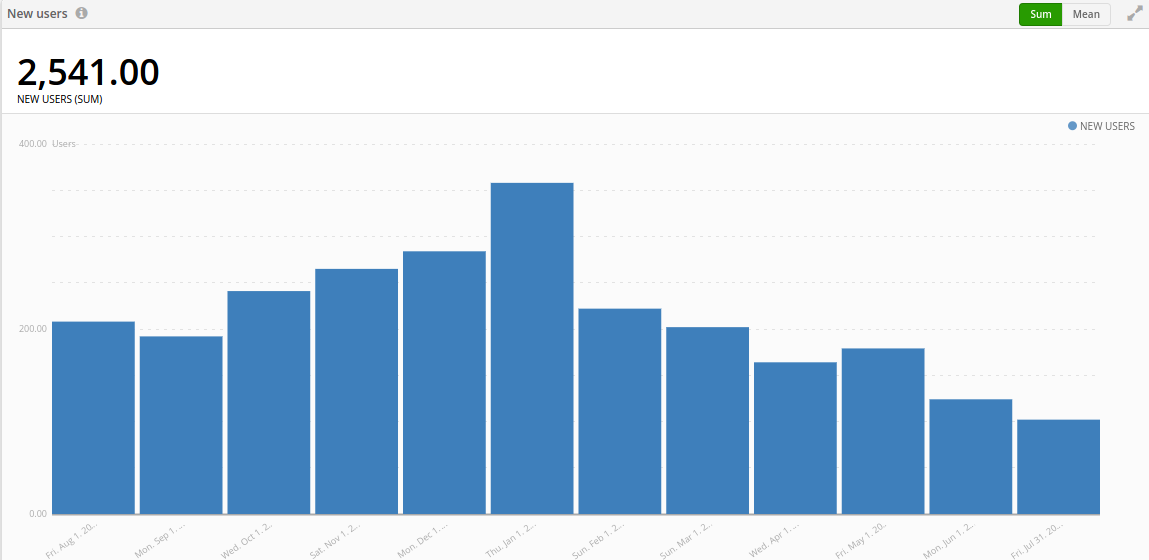
\includegraphics[width=350pt]{graphics/evaluation/bars_users_year.png}
\caption{New users in the first year from release}
\label{fig:bars-first-year}
\end{figure}

As wee can see, we got 2541 users in the first year. Every month the users increased an average of 200 new people. Also, we can observe that there is an evident increase of new users in the months of December and January, which is consequence of the increase of the physical packs sells within Christmas days.

In Figure \ref{fig:bars-all-year} we can see the new users obtained in the whole time our application have been on the market:

\begin{figure}[h]
\centering
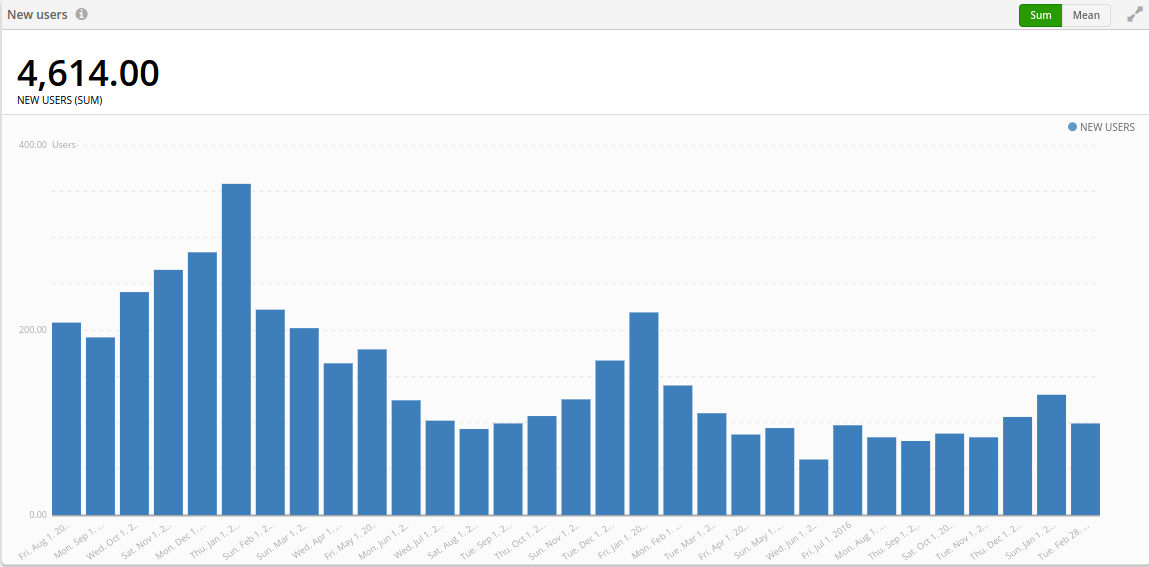
\includegraphics[width=350pt]{graphics/evaluation/bars_users_all.png}
\caption{New users since application first release}
\label{fig:bars-all-year}
\end{figure}

\FloatBarrier

As wee can see, we got 4641 users since our application first release. Also, we can observe that after first year new installations have been decreasing with the exception of the Christmas months described earlier. Even so, during 2016 our game has been constantly downloaded by an average of 100 new users.

\subsection{Users location}

Due to the physical instrument pack is sold in the countries list in the Table \ref{tab:countries}, is very useful to observe new user distribution across the world.

\begin{table}[!htpb]
\centering
    \begin{tabular}{|c|c|c|c|c|}
	\hline
	Argentina & Bulgaria & Colombia & Greece & Hungary \\
	\hline
	Israel & Latvia & Mexico & Poland & Qatar \\
	\hline
	Romania & Saudi Arabia & Switzerland & United Arab Emirates & Uruguay \\
	\hline
	Azerbaijan & China & France & Holland & ~\\
	\hline
	Italy & Lithuania & Peru & Portugal & ~\\
	\hline
	Russia & Spain & Turkey & United States & ~\\
    \hline
    \end{tabular}
\caption{Countries were the physical instrument pack is sold}
\label{tab:countries}
\end{table}

\FloatBarrier

In Figure \ref{fig:map-first-year} we can see the world distribution map of users engaged in the first year:

\begin{figure}[h]
\centering
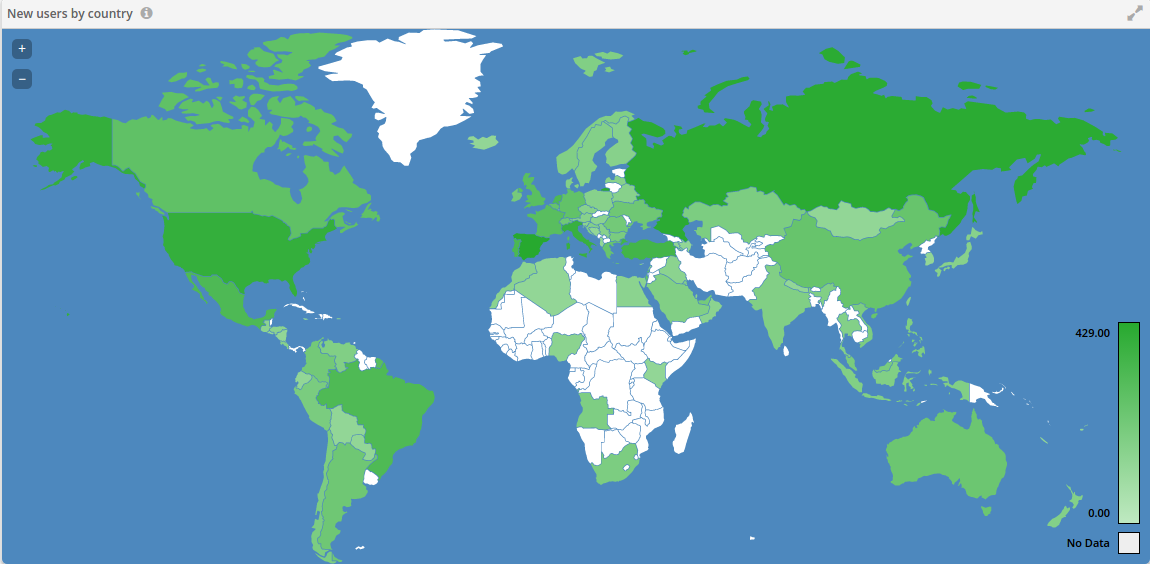
\includegraphics[width=350pt]{graphics/evaluation/map_users_year.png}
\caption{New users location in the first year from release}
\label{fig:map-first-year}
\end{figure}

Also, in Figure \ref{fig:chart-first-year} we can observe the top four countries where the game have been downloaded within this period:

\begin{figure}[h]
\centering
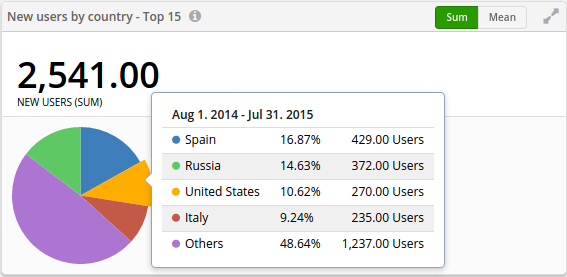
\includegraphics[width=200pt]{graphics/evaluation/chart_users_year.png}
\caption{New users location in the first year from release top countries}
\label{fig:chart-first-year}
\end{figure}

\FloatBarrier

As we can see, the application have been installed from most of the countries located in Europe and America, as long as many countries located in Asia. Also, Spain, Russia, USA and Italy are the countries where most of the users came from.

In Figure \ref{fig:map-all-year} we can see the world distribution map of users obtained in the whole time our application have been on the market:

\begin{figure}[h]
\centering
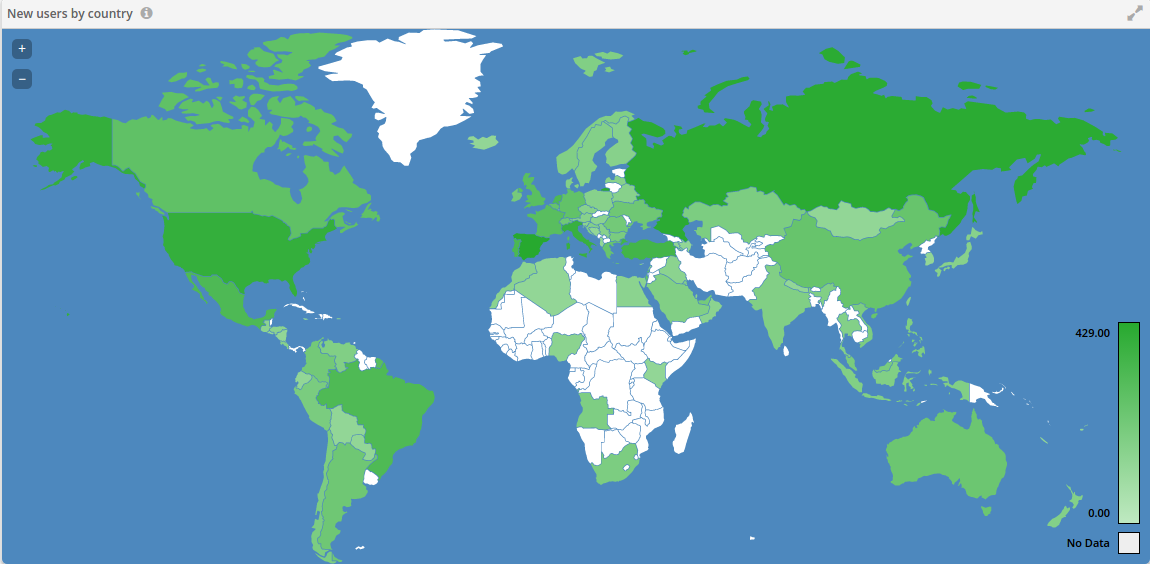
\includegraphics[width=350pt]{graphics/evaluation/map_users_year.png}
\caption{New users location since application first release}
\label{fig:map-all-year}
\end{figure}

Also, in Figure \ref{fig:chart-all-year} we can observe the top four countries where the game have been downloaded within this period:

\begin{figure}[h]
\centering
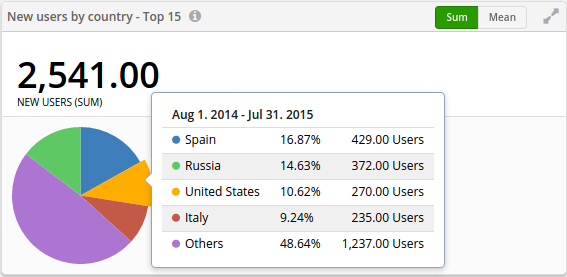
\includegraphics[width=200pt]{graphics/evaluation/chart_users_year.png}
\caption{New users location since application first release top countries}
\label{fig:chart-all-year}
\end{figure}

\FloatBarrier

As we can see, the application have been installed from a few more countries from the ones in the first year. Also, Spain, Russia, USA and Italy are the countries where most of the users came from.

\section{Engagement}

Mobile engagement is the act of engaging a user through available messaging channels inside and outside of an app. Because of that, engagement is such an important metric to analyze if the gamer has considered our application useful as their keep using it.

We will observe user engagement since our game is in the market and through two principal blocks of metrics, user retention and DAU, WAU and MAU metrics.

\subsection{Retention}
Retention is arguably the most important metric in a free-to-play game. Successful free-to-play games create long-term relationships with users. Users that enjoy the experience enough are willing to pay to for a competitive advantage. A game needs to have strong retention to have time to build this relationship.

To calculate retention, separate your users into cohorts based on the day they download your app. The day that the download occurs is Day 0. If a user opens your app the next day (Day 1), they are marked as retained. If they do not open the app, they are not retained. This calculation is performed for user cohort on each day after they download the app. Common days used for retention are 1, 3, 7 and 30.~\cite{gametrics2}

In Figure \ref{fig:app-retention} we can see our game 90 day retention since its release:

\begin{figure}[h]
\centering
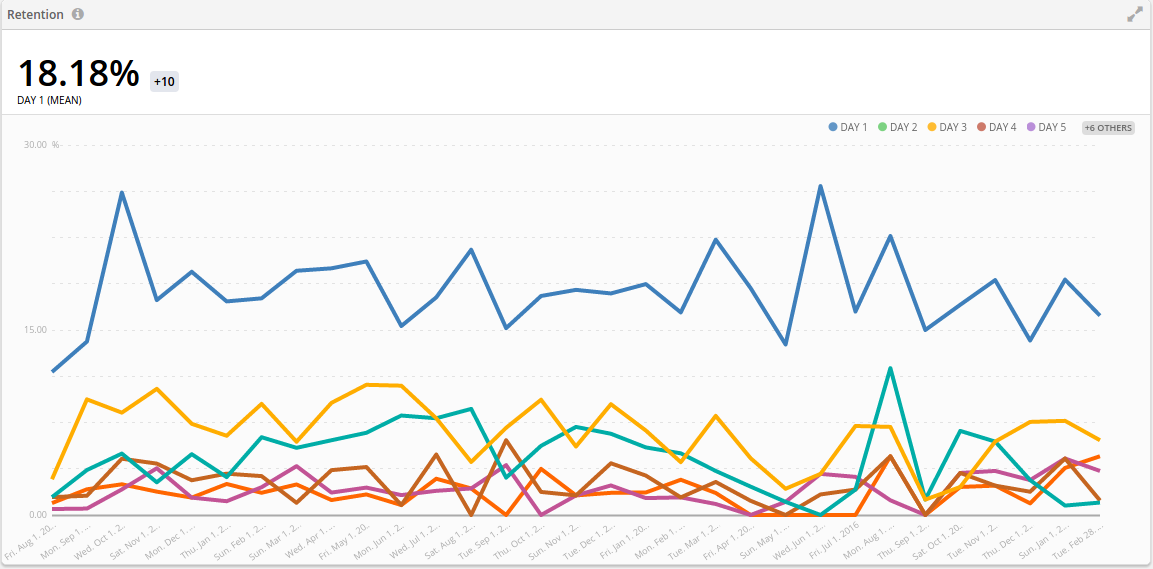
\includegraphics[width=350pt]{graphics/evaluation/app_retention.png}
\caption{Application retention}
\label{fig:app-retention}
\end{figure}

\FloatBarrier

As we can see, our game retention is 18.18\%. Usually, game applications tend to have lower retention values, and  according to Flurry studies, 8\% retention rate at 30 days is average across the kids game iOs sub-category applications.~\cite{flurry2} In our case, we have duplicate generally retention rates for our type of application.

\subsection{DAU, WAU and MAU}

Daily Active Users (DAUs) is the number of unique users that start at least one session in your app on any given day. By themselves, DAU and other high level metrics don’t provide much insight into an app’s performance. However, knowing these simple metrics is a useful starting point for an educated analytics discussion.

Weekly Active Users (WAUs) is the number of unique users that start at least one session in your app on any given week. Having both DAU and WAU, we can obtain the ratio of Daily Active Users to Weekly Active Users.

Monthly Active Users (MAUs) is the number of unique users that start at least one session in your app on any given month. Having both DAU and MAU, we can obtain the ratio of Daily Active Users to Monthly Active Users shows how well an app retains users and is often referred to as the stickiness of a game. This metric shows you how frequently users log in to your app.

Popular social networking apps like Facebook have reported DAU/MAU ratios as high as 50 percent. But most successful gaming apps have ratios closer to 20 percent.~\cite{gametrics2}

In Figure \ref{fig:app-dau} we can see our DAU, WAU and MAU data:

\begin{figure}[h]
\centering
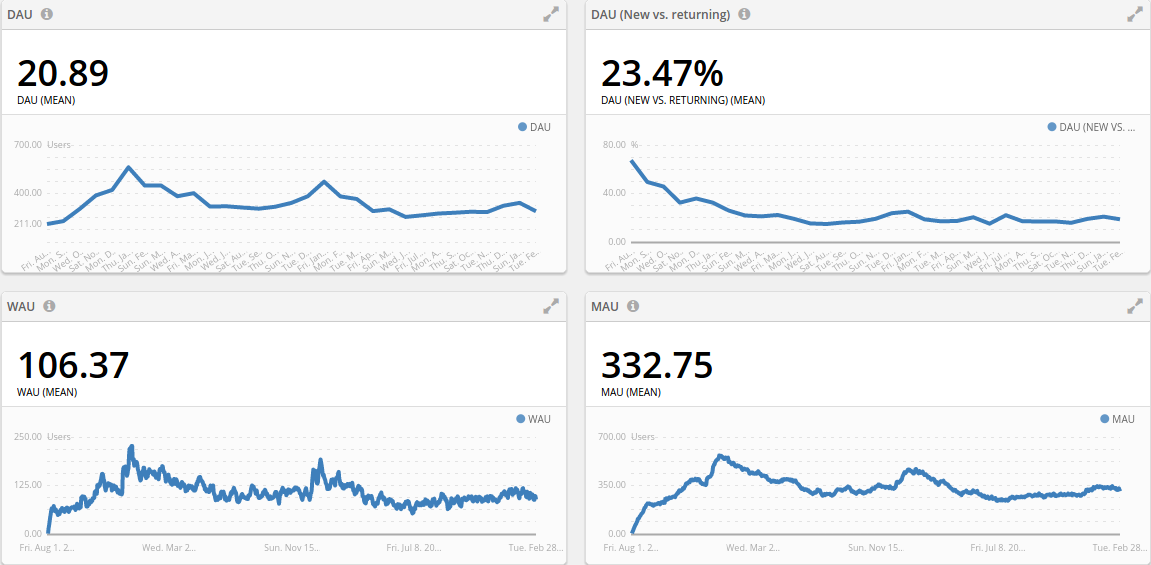
\includegraphics[width=350pt]{graphics/evaluation/app_dau.png}
\caption{Application retention}
\label{fig:app-dau}
\end{figure}

\FloatBarrier

As we can see, if we calculate the DAU/WAU and DAU/MAU ratios, we obtain 20\% and 6\%. This means that the average user logged in on roughly 6 percent of the days that month.

\subsection{Quality}

We will study our game quality in terms of the average numbers of screens the levels plays and in the average of frames per second their devices give.

In Figure \ref{fig:app-levels} we can see the mean of levels that our gamers plays in every month since the application release.

\begin{figure}[h]
\centering
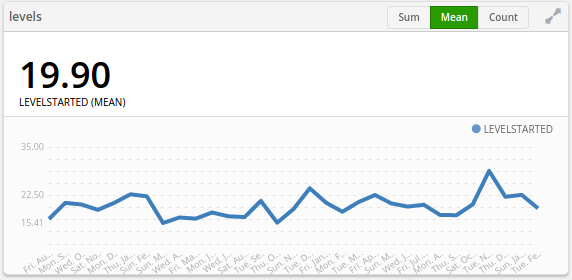
\includegraphics[width=250pt]{graphics/evaluation/app_levels.png}
\caption{Application levels average}
\label{fig:app-levels}
\end{figure}

\FloatBarrier

As we can see, gamers plays an average of 20 levels per month. In our case, each screen is a level, so the gamer plays thorough at least 20 different screens each month.

Finally, in Figure \ref{fig:app-fps} we can observe the average frames per second shown by gamers devices. 

\begin{figure}[h]
\centering
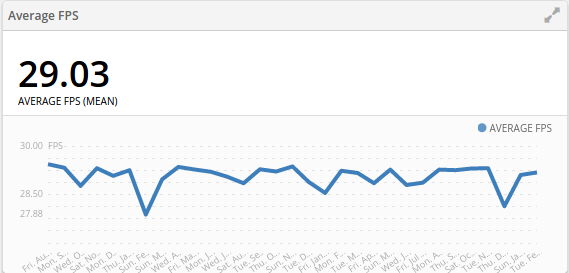
\includegraphics[width=250pt]{graphics/evaluation/app_fps.png}
\caption{Application fps average}
\label{fig:app-fps}
\end{figure}

\FloatBarrier

As we can see, gamers devices shown an average of 29 frames per second, which is the estimated value for a game which manages lots of audio and animation resources.

\subsection{Summary}
In this chapter we evaluated our application using the metrics available from Unity Game Analytics.

Firstly, we observe user acquisition in order to study the numbers of new users we obtained during the first year of the application in the market and since its release. Also, we took a look at the users location distribution.

Secondly, we detailed user engagement so that we can know if the users tend to use our game after its installation. We took a look at retention information since application release as long as DAU, WAU and MAU metrics.

Finally, we observed the game quality detailed the numbers of levels the gamer played and the numbers of frames per second their devices shown since the application release.


